\section{Data and Analysis}
\label{sec:data}

\subsection{RQ1 Analysis}
In RQ1, we evaluate  GTXCrawler ability to see 
if it can accurately detect the relationship 
between the classes to the test cases. 
To do this, we compared the results of applying GTXCrawler
with Jaccard Index technique, which is a commonly used
technique for calculating the term similarity in test suite~\cite{noor15}.
We choose Jaccard Index because the previous study 
shown that this technique is a better term similarity indicator
than other techniques~\cite{mondal15}. 

To evaluate the effectiveness of GTXCrawler, we used 
common accuracy indicators to determine the accuracy of
our model. The three accuracy indicators that we used are
precision (Prec.), Recall and F-Measure (FM). 
Prec indicates the percentage of correctly
classified instances, Recall indicates the percentage 
of correctly selected test cases that are relevant to the 
modified source file, 
and FM is the weighted average of Precision and Recall. 
We randomly select 20 percent of 
the test cases as a test dataset and 60 percent as 
a training dataset and 20\% as validation set.


Table~\ref{tab:recall} shows the average 
results for each application. 
The results show that the Recall, 
Precision and F-measure achieved by GTXCrawler 
is statistically higher than that achieved by Jaccard Index
in most cases. 
Only in four out of fifteen cases 
Jaccard Index achieved higher f-Measure
(Umbraco-CMS v7.7.2, Joda-Time v1.2, 
Joda-Time v1.3 and Joda-Time v1.4).
Therefore, we can conclude that GTXCrawler is
a better tractability link indicator than
Jaccard Index. 





\begin{table*}[!ht]
	\caption{Accuracy Results Achieved Using GTXCrawler Versus Jaccard Index.}
	\vspace*{-10pt}
	\begin{center}
		{\scriptsize
			\begin{tabular}{|c|c|c|c||c|c|c|}\hline
				Application & \multicolumn{3}{c||} {GTXCrawler}  & \multicolumn{3}{c|} {Jaccard Index} 
				\\\hline & Prec. (\%)  & Recall(\%) & FM (\%)& Prec. (\%)  & Recall(\%) & FM (\%) \\\hline \hline				
				
			    nopCommerce	v2.10 &	88 & 76 & 81 &	69 & 52 & 59 \\
				nopCommerce v2.30 &	81 & 77	& 78 & 67 & 71 & 69	\\
				Umbraco-CMS v7.7.2 & 74 & 80 & 76 & 80	& 77 & 78 \\
				Umbraco-CMS v7.7.5 & 83 & 81 & 82 & 79 & 74	& 76 \\
				Joda-Time v0.95 & 77 & 72 & 74	& 57 & 59 & 58 \\
				Joda-Time v0.99 & 72 & 76 & 74	& 66 & 72 & 69 \\
				Joda-Time v1.2 & 69 & 63 & 66 &	73 & 78	& 75 \\
				Joda-Time v1.3 & 80 & 72 & 75 & 85 & 81	& 83 \\
				Joda-Time v1.4 & 81 & 78 & 80 &	84 & 80	& 82 \\
				Joda-Time v1.5 & 80 & 87 & 83 & 59 & 71	& 64 \\
				JFreeChart v1.0.1 &	92 & 92 & 92 & 74 & 65 & 69	\\
				JFreeChart v1.0.3 &	83 & 78 & 80 &	69 & 58	& 63 \\
				JFreeChart v1.0.5 &	 83 & 81 & 82 & 70 & 64	& 67 \\
				JFreeChart v1.0.7 &	 67 & 77 & 72 &	72 & 66 & 69 \\
				JFreeChart v1.0.9 & 79 & 81 & 80 & 63 & 69 & 66 \\\hline 				
					
			\end{tabular}
		}
		\end {center}
		\label{tab:recall}
		\vspace*{-5pt}
	\end{table*}



\subsection{RQ2 Analysis}


Figure~\ref{fig:testselected} shows how many tests need to be selected
by each approach to achieve a given recall average. For instance, in
case of nopCommerce V2.10 our approach requires 251 (0.48\%) 
top-ranked tests to detect 100\%
of the test failures, compared to at least 407 (78\%) tests
when using the total code coverage technique. 
In case of JfreeChart V1.0.7 our approach requires
1,206 (45\%) top-ranked tests to detect 75\% of the 
test failures, compared to at least 1,608 (60\%) tests when using
the Jaccard Index technique.

\begin{figure*}[!ht]
	\centering
	\includegraphics[width=0.90\linewidth]{./testselected.png}
	\vspace*{-3pt}
	\caption{Average percentage of test selected}
	\label{fig:testselected}
	%	\vspace*{-10pt}
\end{figure*}


%%% elaborate more

\subsection{RQ3 Analysis}

RQ3 investigates the applicability of GTXCrawler
in the area of test case prioritization. 
To evaluate the effectiveness of GTXCrawler
we computed the APFD values and compared its 
results with three different prioritization techniques.
Figure~\ref{fig:FDR} shows the APFD results variation.
The horizontal bar shows the prioritization technique
and the vertical bar represent APFD values. 


This experiment was performed 30 times with 
random selections each time. 
APFD values were computed by prioritizing all 
test cases for each application. 
In eleven of the fifteen subject application, prioritization 
by GTXCrawler yielded a higher APFD than other
prioritization techniques.
However, all the APFD values were within a few percentage 
point of each other. 


\begin{figure*}[!hb]
	\minipage{0.33\textwidth}
	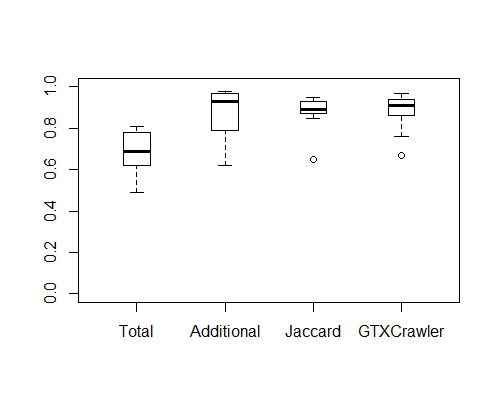
\includegraphics[width=0.95\linewidth]{./nop1.png}
	\caption*{nopCommerce V2.10}
	\label{fig:nop1}
	\endminipage\hfill
	\minipage{0.33\textwidth}
	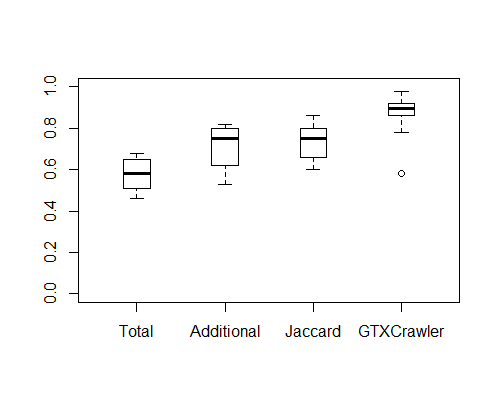
\includegraphics[width=0.95\linewidth]{./nop2.png}
	\caption*{nopCommerce V2.30}
	\label{fig:nop2}
	\endminipage\hfill
	\minipage{0.33\textwidth}
	\includegraphics[width=0.95\linewidth]{./umbra1.png}
	\caption*{Umbraco V7.7.2}
	\label{fig:umbra1}
	\endminipage\hfill		
    \vspace*{-10pt}	
\end{figure*}

\begin{figure*}[!hb]
	\minipage{0.33\textwidth}
	\includegraphics[width=0.95\linewidth]{./umbra2.png}
	\caption*{Umbraco V7.7.5}
	\label{fig:umbra2}
	\endminipage\hfill
	\minipage{0.33\textwidth}
	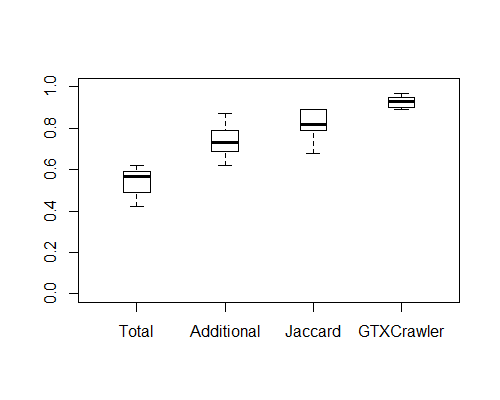
\includegraphics[width=0.95\linewidth]{./joda1.png}
	\caption*{Joda-Time V 0.95}
	\label{fig:joda1}
	\endminipage\hfill	
	\minipage{0.33\textwidth}
	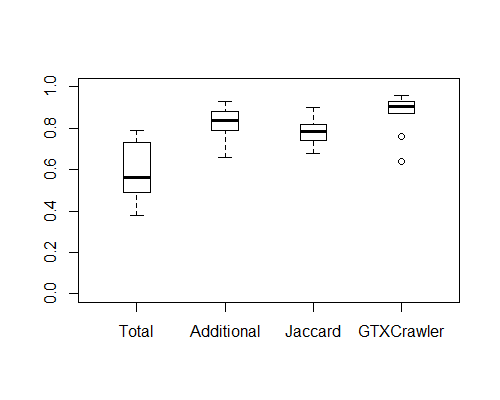
\includegraphics[width=0.95\linewidth]{./joda2.png}
	\caption*{Joda-Time V 0.99}
	\label{fig:joda2}
	\endminipage\hfill	
\end{figure*}

\begin{figure*}[!hb]
	\minipage{0.33\textwidth}
	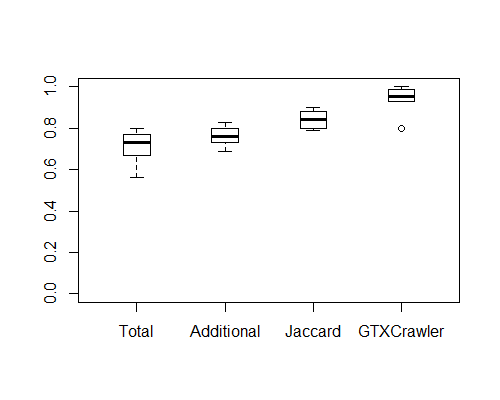
\includegraphics[width=0.95\linewidth]{./joda3.png}
	\caption*{Joda-Time V 1.2}
	\label{fig:joda3}
	\endminipage\hfill		
	\minipage{0.33\textwidth}
	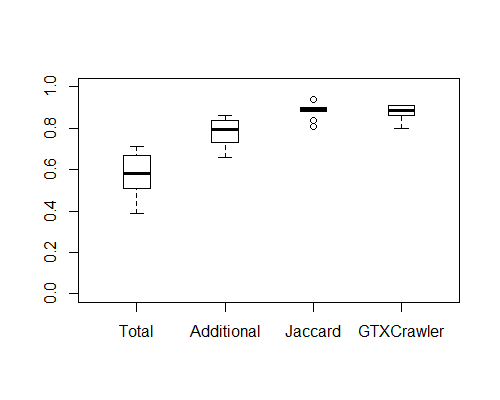
\includegraphics[width=0.95\linewidth]{./joda4.png}
	\caption*{Joda-Time V 1.3}
	\label{fig:joda4}
	\endminipage\hfill
	\minipage{0.33\textwidth}
	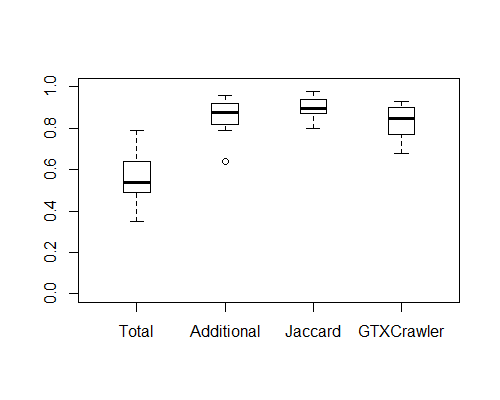
\includegraphics[width=0.95\linewidth]{./joda5.png}
	\caption*{Joda-Time V 1.4}
	\label{fig:joda5}
	\endminipage\hfill
\end{figure*}

\begin{figure*}[!hb]
	\minipage{0.33\textwidth}
	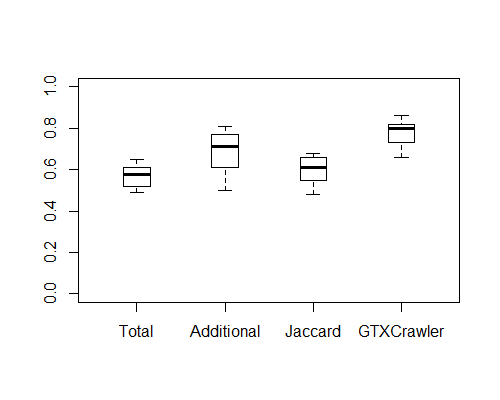
\includegraphics[width=0.95\linewidth]{./joda6.png}
	\caption*{Joda-Time V 1.5}
	\label{fig:joda6}
	\endminipage\hfill
	\minipage{0.33\textwidth}
	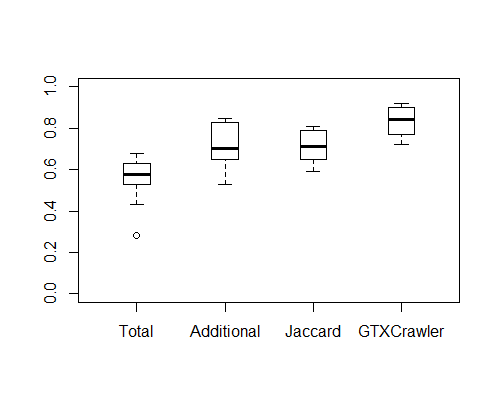
\includegraphics[width=0.95\linewidth]{./jfree1.png}
	\caption*{JfreeChart V1.0.1}
	\label{fig:jfree1}
	\endminipage\hfill		
	\minipage{0.33\textwidth}
	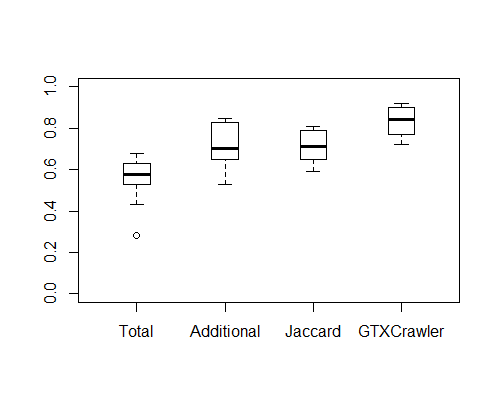
\includegraphics[width=0.95\linewidth]{./jfree1.png}
	\caption*{JfreeChart V1.0.3}
	\label{fig:jfree2}
	\endminipage\hfill	
\end{figure*}

\begin{figure*}[!hb]	
	\minipage{0.33\textwidth}
	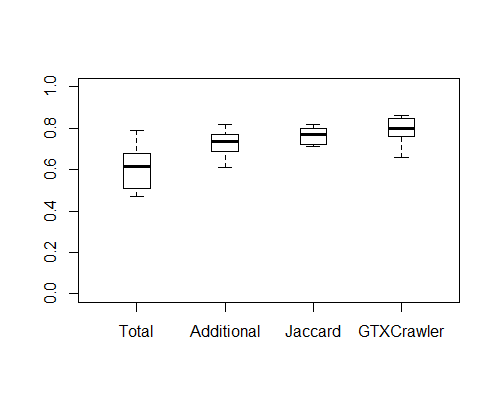
\includegraphics[width=0.95\linewidth]{./jfree3.png}
	\caption*{Joda-Time V 1.0.5}
	\label{fig:jfree3}
	\endminipage\hfill
	\minipage{0.33\textwidth}
	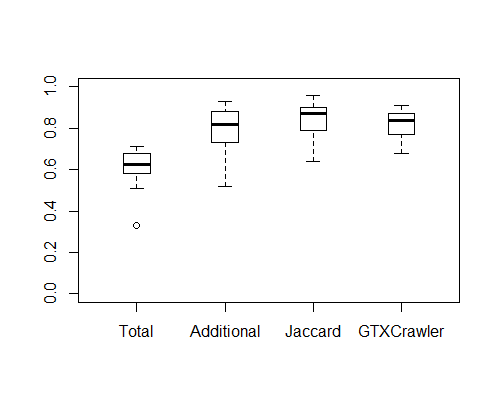
\includegraphics[width=0.95\linewidth]{./jfree4.png}
	\caption*{Joda-Time V 1.0.7}
	\label{fig:jfree4}
	\endminipage\hfill
	\minipage{0.33\textwidth}
	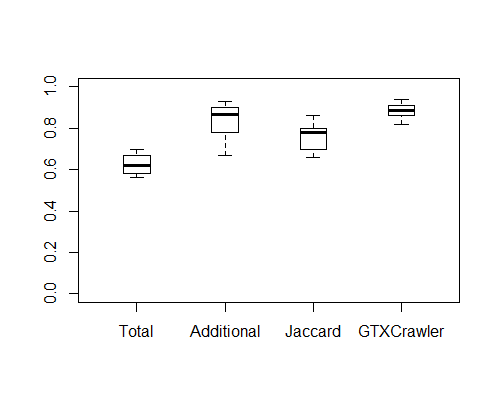
\includegraphics[width=0.95\linewidth]{./jfree5.png}
	\caption*{JfreeChart V1.0.9}
	\label{fig:jfree5}
	\endminipage\hfill		
%	\minipage{0.24\textwidth}
%	\includegraphics[width=0.95\linewidth]{./plain.png}
%	\caption*{}
%	\label{fig:jfree6}
%	\endminipage\hfill
	\caption{Mean percentage of faults detected over time, where time is shown in percentage of total execution time of all the test cases, in the test suite. The error bars correspond to the 95\% confidence interval.}	
	\label{fig:FDR}	
	\vspace*{-40pt}
\end{figure*}

